\documentclass{article}
\usepackage[utf8]{inputenc}
\usepackage[russian]{babel}
\usepackage[left=2cm,right=2cm,top=2cm,bottom=2cm,bindingoffset=0cm
]{geometry}
\usepackage{cmap}
\usepackage{fancyvrb}
\usepackage{graphicx}
\graphicspath{{pictures/}}
\DeclareGraphicsExtensions{.pdf,.png,.jpg}
\DefineShortVerb{\|}

\begin{document}

\begin{titlepage} \begin{center}

	\Large			
Санкт-Петербургский политехнический университет Петра Великого
			
	\vspace{0.2cm}	
Институт компьютерных наук и технологий
		
	\vspace{2cm} \vfill \huge
Проект OWASP WebGoat
		
	\vfill 
	\begin{flushleft} \large \hangindent=8cm \hangafter=0
Выполнил: Сухинин А.А. гр. 53501/3 \hrulefill
			
Принял: Выглежанина К.Д. \hrulefill
	\end{flushleft}
		
	\vspace{2cm} \vfill \LARGE
2015 г.
		
\end{center} \end{titlepage}

\section{Ход работы}
\subsection{Изучение}

\paragraph{Изучить описания десяти самых распространенных веб-уязвимостей согласно рейтингу OWASP}

\begin{enumerate}
\item SQL инъекция. Следует использовать prepared statements или экранирование для избежания данной проблемы. Можно получить практически полный доступ к БД.
\item Нарушение авторизации и управления сессией. Данная информация никогда не должна передаваться в открытом виде.
\item Отсутствие экранирования входных параметров. Это может привести к выполнению вредоносных скриптов на клиентах.
\item Отсутствие проверки прав пользователя при доступе к ресурсам.
\item Неправильная настройка (пароли по умолчанию, необновленное ПО, вывод stack trace и т.п.)
\item Хранение важной информации (пароли, данные кредитных карточек) хранятся в открытом виде в течение длительного периода или передаются по недостаточно защищенному соединению.
\item Missing Function Level Access Control (частный случай 4 пункта)
\item Уязвимость к кроссдоменным запросам. Атакующий может вставить запрос к приложению на собственном ресурсе. Если жертва уже авторизована, то это может привести к исполнению вредоносного запроса. Для избежания этого необходимо вместе с запросом передавать уникальный для сессии токен.
\item Использование уязвимых компонентов (Apache CXF Authentication Bypass, Spring Remote Code Execution)
\item Незащищенные перенаправления и forwarding (как по русски?)
\end{enumerate}

\subsection{Практическое задание}

Запустить уязвимое приложение WebGoat. Запустить сканер безопасности ZAP. Запустить инструмент Mantra, настроить его для использования ZAP в качестве прокси-сервера
\paragraph{Недостатки контроля доступа}
~

\begin{enumerate}
\item Bypass Bussines Layer Access.

Для выполнения данного задания нужно включить прокси и авторизоваться за пользователя имеющего права удаления. Используя прокси просмотреть параметры запроса для удаления.

Затем для пользователя, не имеющего указанные права перехватить пакет и передать в качестве параметра нужную операцию.

\begin{verbatim}
employee_id=105&action=DeleteProfile
\end{verbatim}


\item Bypass Data Layer Access

В данном примере все проще. Необходимо перехватить пакет и подменить в нем id запрашиваемого пользователя.
\begin{verbatim}
employee_id=104&action=ViewProfile
\end{verbatim}
\end{enumerate}

\paragraph{Безопасность AJAX}
~

\begin{enumerate}
\item Dom based cros-site scripring

В данном примере можно наблюдать уязвимости, открывающиеся перед злоумышленником, если не экранировать входные данные.

Для защиты от данной уязвимости необходимо использовать функцию escapeHTML().

\item Same origin Policy Protection. 

Данная политика безопасности позволяет запускать скрипты только с того же домена.

\item Client Side Filtering. 

В данном уроке демонстриется уязвимость, связанная с тем, что данные фильтруются на клиентской строне. Для избежания данной уязвимости, данные необходимо фильтровать еще до отправки.
 
Пример ответа на запрос:
\begin{verbatim}
<table align='center' cellspacing='0' width='90%' border='1' cellpadding='0'><tr><td>UserID</td>
<td>First Name</td><td>Last Name</td>
<td>SSN</td><td>Salary</td></tr><tr id='101'>
<td>101</td><td>Larry</td><td>Stooge</td>
<td>386-09-5451</td><td>55000</td></tr>
<tr id='102'><td>102</td><td>Moe</td>
<td>Stooge</td><td>936-18-4524</td><td>140000</td></tr>
<tr id='103'><td>103</td><td>Curly</td>
<td>Stooge</td><td>961-08-0047</td>
<td>50000</td></tr><tr id='104'><td>104</td><td>Eric</td>
<td>Walker</td><td>445-66-5565</td>
<td>13000</td></tr><tr id='105'><td>105</td>
<td>Tom</td><td>Cat</td><td>792-14-6364</td><td>80000</td></tr>
<tr id='106'><td>106</td><td>Jerry</td>
<td>Mouse</td><td>858-55-4452</td><td>70000</td></tr>
<tr id='107'><td>107</td><td>David</td>
<td>Giambi</td><td>439-20-9405</td><td>100000</td></tr>
<tr id='108'><td>108</td><td>Bruce</td>
<td>McGuirre</td><td>707-95-9482</td><td>110000</td></tr>
<tr id='109'><td>109</td><td>Sean</td>
<td>Livingston</td><td>136-55-1046</td><td>130000</td></tr>
<tr id='110'><td>110</td><td>Joanne</td>
<td>McDougal</td><td>789-54-2413</td><td>90000</td></tr>
<tr id='111'><td>111</td><td>John</td>
<td>Wayne</td><td>129-69-4572</td><td>200000</td></tr>
<tr id='112'><td>112</td><td>Neville</td>
<td>Bartholomew</td><td>111-111-1111</td><td>450000</td></tr></table>

\end{verbatim} 
 
Правильная фильтрация:
\begin{verbatim}
	sb.append("/Employees/Employee/ [Managers/Manager/text()='" + userId +"']/UserID | ");
	sb.append("/Employees/Employee/ [Managers/Manager/text()='" + userId +"']/FirstName | ");
	sb.append("/Employees/Employee/ [Managers/Manager/text()='" + userId +"']/LastName | ");
	sb.append("/Employees/Employee/ [Managers/Manager/text()='" + userId +"']/SSN | ");
	sb.append("/Employees/Employee/ [Managers/Manager/text()='" + userId +"']/Salary ");
\end{verbatim} 

\item DOM injection

Для этого в документ необходимо добавить строку:
document.forms[0].SUBMIT.disabled=false;

\item XML Injection

При посылке запроса необходимо добавить:
\begin{verbatim}
<root>
<reward>WebGoat Mug 20 Pts</reward>
<reward>WebGoat t-shirt 50 Pts</reward>
<reward>WebGoat Secure Kettle 30 Pts</reward>
<reward>WebGoat Core Duo Laptop 2000 Pts</reward>
<reward>WebGoat Hawaii Cruise 3000 Pts</reward>
</root>
\end{verbatim}


\item JSON Injection

При посылке необходимо изменить ответ на:

\begin{verbatim}
{
"From": "Boston",
"To": "Seattle", 
"flights": [
{"stops": "0", "transit" : "N/A", "price": "$20"},
{"stops": "2", "transit" : "Newark,Chicago", "price": "$300"} 
]
}
\end{verbatim}

\item Sielent tansactions attack

Очередной урок на тему того, что не нужно делать проверки на клиентской строне. Находим клиентскую функцию для отправки, вызываем ее.

submitData(555, 1000000)

\item Insecure client srorage

Очередное!

Снимаем флажки readonly, ставим карточку GOLD, обнуляем стоимость покупок.

\item Dangerous use of eval

eval вообще крайне не рекомендуется использовать, но чтобы так вот. Для выполнения задания нужно ввести в поле
\begin{verbatim}
')%3Balert(document.cookie%2B'something
\end{verbatim}

\end{enumerate}

\paragraph{Недостатки аутентификации}
~

\begin{enumerate}
\item Password strength

На сервисе howsecureismypassword.net можно узнать примерное время взлома пароля. Вместе длиной пароля очень быстро растет время его подбора.

\item Forgot password

Сложность восстановления пароля должна быть сопоставима с подобором пароля, иначе это бессмысленно.

\item Multi level login 1

Перехватываем пакет, выставляем hiddentan=1. Смысл использовать многоуровневую защиту, если по факту она не реализована?

\item Multi level login 2

Авторизуемся за Joe, вводим его tan, перехватываем сообщение и в запросе указываем Jane. (!!!!)
\begin{verbatim}
Results:
Username: admin
Color: green
Password: 2275$starBo0rn3
\end{verbatim}
\end{enumerate}

\paragraph{Переполнение буффера}
~

Перехватываем пакет, в поле roomno вбиваем >4086 символов. Идем до конца. После регистрации посматриваем скрытые поля. Выбираем одного из них. Заходим от его имени для завершения.

\begin{verbatim}
<input type="HIDDEN" value="Hamilton" name="a"></input>
<input type="HIDDEN" value="Lewis" name="b"></input>
<input type="HIDDEN" value="9901" name="c"></input>
\end{verbatim}

\paragraph{Качество кода}
~

При просмотре страницы можно обнаружить запись в комментариях admin:adminpw. Это и является логином и паролем администратора. (!!)

\paragraph{Многопоточность}
~

\begin{enumerate}
\item Thread safety problem

При одновременном получении данных пользователя возможна утечка. Используя эту уязвимость можно получить чужие данные. Открываем два окна вводим имена пользователей. В некоторых ситуациях можем получить не свою информацию.

\item Shopping cart Concurrency flew

Открываем два окна, в одном делаем большую покупку, в другом - маленькую. Продолжаем дешевую покупку, обновляем большую. При подтверждении оплачиваем небольшую сумму, но получаем большую покупку.
\end{enumerate}

\paragraph{Межсайтовое выполнение сценариев}
~

\paragraph{Неправильная обработка ошибок}
~

Перехватываем пакет, удаляем передаваемый параметр "пароль". Успешная авторизация! (!!!!)

\paragraph{Недостатки приводящие к осуществлению инъекций}
~

\begin{enumerate}
\item Command injection

Перехватываем запрос, добавляем к имени файла строку:
\begin{verbatim}
%22%3B%20netstat%20-a
\end{verbatim}

\item Numeric SQL injection

Перехватываем запрос. Модифицируем:

\begin{verbatim}
station=101or%201%3D1&SUBMIT=Go!
\end{verbatim}

\item Log spoofing

Перехватываем запрос, меняем имя на следующее:
\begin{verbatim}
somename
Admin succefully entered!
\end{verbatim}

В результате, в логе создается видимость того, что админ авторизоавлся.

\item XPath Injection 

К имени добавляем:
\begin{verbatim}
' or 1=1 or 'a'='a
\end{verbatim}

Почему-то не работает без or 1=1

\item SQL Injection

Перехватываем сообщение. В качестве пароля вводим:
\begin{verbatim}
azaza%27%20OR%20%271%27%3D%271
\end{verbatim}

При попытке получить данные на втором шаге получаем сообщение:
\begin{verbatim}
THIS LESSON ONLY WORKS WITH THE DEVELOPER VERSION OF WEBGOAT
\end{verbatim}

\item String sql injection

Аналогично. Вместо имени вводим azaza' OR 'a' = 'a. Получаем все возможные значения.

\end{enumerate}

\paragraph{Отказ в обслуживании}
~

\begin{enumerate}
\item ZipBomb 

Cоздаем архив с файлом содержащим одинаковые символы. Такой файл обладает очень высоким коэф. сжатия. Посылаем. При распаковке требуется очень много места.

\item Denial of Service from Multiple Logins

Используем инъекцию для получения паролей. Вместо пароля пишем:
\begin{verbatim}
"dont_care' or '1' = '1"
\end{verbatim}

Получаем таблицу:
\begin{verbatim}
101	jsnow	passwd1	
102	jdoe	passwd2	
103	jplane	passwd3	
104	jeff	jeff	
105	dave	dave	
\end{verbatim}

Используем полученные результаты для авторизации. Из-за большого количества сессий получаем отказ в обслуживании.

\end{enumerate}

\paragraph{Небезопасное сетевое взаимодействие}
~

Перехватываем пакет. Извлекаем из аргумента password пароль. Меняем соединение на защищенное. Пароль недоступен, одно видны параметры соединения. TLS, текст закрыт.

\paragraph{Небезопасная конфигурация}
~

Приложение не настроено должным образом. Если знать адрес интерфейса администрирования, можно получить к нему доступ под собственными паролями.

Расположено по адресу WebGoat/conf.

\paragraph{Небезопасное хранилище}
~

Есть возможность попробовать различные строки и увидеть особенности кодировки строк различными алгоритмами.

\paragraph{Исполнение злонамеренного кода}
~

Если на сервере неправильно настроены директории для сканирования скриптов, можно загрузить собственный исполняемый файл, перейти на интересующую старицу и выполнить злонамеренный код.

Содержимое файла attack.jsp
\begin{verbatim}
<HTML>
<%
java.io.File file = new java.io.File("C:\\Users\\llama\\Desktop\\secure\\.extract\\webapps\\WebGoat\\mfe_target\\webgoat.txt");
file.createNewFile();
%>
</HTML>
\end{verbatim}

\paragraph{Подделка параметров}
~

\begin{enumerate}
\item Bypas HTML Field Restrictions 

Перехватываем сообщение. Меняем все поля. Добавляем disabledinput.

\item Exploit Hidden Fields

Перехватываем, меняем...

\item Exploit unchecked email

Отправляем сообщение типа:
\begin{verbatim}
<script>alert("Bad Stuff");</script>
\end{verbatim}

Для отправки сообщения friend перехватываем сообщение меняем параметр "to" чтобы получилось: 
\begin{verbatim}
gId=GMail+id&gPass=password&subject=Comment+for+WebGoat&to=webgoat.admin
%40owasp.org&msg=%3Cscript%3Ealert(%22Bad+Stuff%22)%3B%3C%2Fscript%3E&SUBMIT=Send!
\end{verbatim}

\item Bypass Client Side JavaScript Validation

Аналогично.
\end{enumerate}

\paragraph{Недостатки управления сессией}
~

\begin{enumerate}

\item Подделка сессии. Перехватываем два ключа.

\begin{verbatim}
webgoat 65432ubphcfx
aspect  65432udfqtb
\end{verbatim}

На самом деле эти ключи получаются добавлением к строке 65432 инвертированного имени со смещением букв +1. Для пользователя alice это 65432fdjmb.

Далее перехватываем пакеты, добавляем поле в заголовок Cookie AuthCookie=65432fdjmb

\item HiJack a session

Похожим образом, только намного сложнее закручено.

\item Session fixation

В версии 6.0.1 не работает. Основная идея вынудить жертву пройти по ссылке, которая установит значение session id. Затем как в предыдущем случае использовать этот известный номер для авторизации от имени жертвы. В данной версии переход по ссылке ничего не дает.
\end{enumerate}

%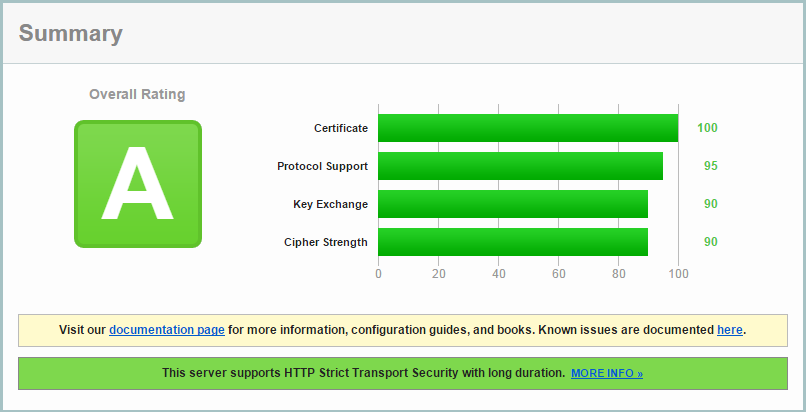
\includegraphics[width=\linewidth]{good}
%\begin{center}
%Рис. 2. Summary recent best.
%\end{center}


\section{Выводы}

В ходе данной работы были изучены "best practice" использования SSL/TLS. Были рассмотрены основные возможности сервиса Qualys SSL Labs – SSL Server Test. Данный сервис позволяет провести анализ качества защищенности домена. В качестве резюме можно получить статус самых известных уязвимостей для данной сервера, а также информацию о поддерживаемых протоколах и режимах работы. Кроме того, сервис тут же предлагает дополнительную информацию по вопросам решения указанных проблем. 

В качестве вывода, можно отметить важность анализа конфигурации SSL/TLS, особенно, при коммерческом использовании. Данный анализ можно удобно выполнить при помощи данного инструмента, однако если требуется особенно тщательная проверка, то она должна быть проведена дополнительно.
 
\end{document}